\subsection{Le Process Hitting }

Dédié la modélisation de grands systèmes complexes, le Process Hitting permet de représenter les modèles possédant une structure simple dont nous prenons avantage pour le développement d’analyses statiques efficaces. Le Process Hitting regroupe un nombre fini de processus (chacun étant biologiquement équivalent à un niveau) séparés en un ensemble de sortes (dont chacune représente un composant biologique). À tout instant, un et un seul processus de chaque sorte est présent (autrement dit chaque composant biologique a un niveau à chaque instant). Un processus peut être remplacé par un autre processus de même sorte par la frappe d’un autre processus présent ce qui se traduit par le changement de niveaux des composant après une certaine réaction. Particulièrement adapté à la modélisation des RRB, le Process Hitting permet une construction simple de la
dynamique généralisée des RRB.

\subsubsection{Réseau de régulation biologique }
Les phénomènes de régulation jouent un rôle crucial dans de nombreux systèmes biologiques,
tel la production des protéines au sein d’une cellule. La figure \ref{cellule} schématise le phénomène de
régulation génique : quand un gène est exprimé, il produit, à travers un processus de transcription
et de traduction, une protéine, qui peut avoir un effet d’activation ou d’inhibition sur l’expression d’un
autre gène, accélérant ou freinant ainsi la production d’autres protéines (ou sa propre production).\\
\begin{figure}[!ht]
    \center
    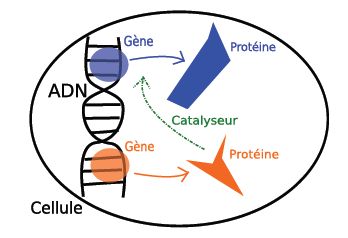
\includegraphics[width=0.5\textwidth]{./images/cellule.png}
    \caption{Schéma d’un phénomène de régulation au sein d’une cellule \cite{pauleve2011modelisation} : un gène produit une
protéine (à travers un processus biologique complexe) qui a un effet de catalyseur (accélération ou
décélération) sur la production d’une autre protéine.}
    \label{cellule}
\end{figure}

Ces informations qualitatives sur l’influence positive ou négative entre les composants d’un système
biologique sont représentées par un graphe des interactions : On trouve des noeuds qui représentent des entités biologiques (gène, ARN, etc.), et sont reliés par
des arcs orientés positifs ou négatifs dénotant respectivement une activation ou une inhibition. La figure \ref{expThomas} donne un exemple de graphe des interactions.\\
\begin{figure}[!ht]
    \center
    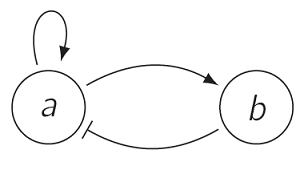
\includegraphics[width=0.5\textwidth]{./images/expThoma.png}
    \caption{Exemple pris de \cite{pauleve2011modelisation} de graphe des interactions d'un RRB ayant deux composants $a$ et $b$ avec un arc activateur de $a$ vers $b$, une auto-activation de noeud $a$ et un arc inhibiteur de $b$ vers $a$.}
    \label{expThomas}
\end{figure}

Ce graphe des interactions constitue une spécification très abstraite d’un RRB et n’indique
pas précisément l’évolution de la concentration des composants en fonction de leurs régulateurs. C'est pour cette raison qu'il y a eu le développement du nouveau formalisme appelé le Process Hitting que nous abordons par la suite.


\subsubsection{Définition du PH}
\label{secDefPH}

la figure \ref{fig:expPH} présente le  Process Hitting(PH)\cite{pauleve2011modelisation}
,qui permet de modéliser un nombre fini de niveaux locaux, appelées processus, regroupés en un ensemble fini d'éléments, appelés sorte. Un processus est noté par $a_i$, où $a$ est le nom de la sorte, et $i$ est l'identifiant du processus dans la sorte. A tout moment, exactement un processus de chaque sorte est actif, et l'ensemble des processus actifs est appelé un état.\\
Les interactions concurrentes entre les processus sont définies par un ensemble d'actions. Ces actions décrivent le remplacement d'un processus par un autre de  la même sorte conditionné par la présence d'au plus un autre processus dans l'état actuel. Une action est notée par $\PHfrappe{a_i}{b_j}{b_k}$, qui est lu comme "$a_i$ frappe $b_j$ pour le faire bondir à $b_k$", où $a_i$, $b_j$, $b_k$ sont des processus de sortes $a$ et $b$, appelées respectivement le \emph{frappeur}, la \emph{cible} et le \emph{bond} de l'action. Nous notons également une \emph{auto-frappe} toute action dont le frappeur et cible sont les mêmes, de la forme: $\PHfrappe{a_i}{a_i}{a_k}$.

\begin{definition}[Process Hitting] (\cite{pauleve2011modelisation})

  Un \emph{Process Hitting} est un triplet  $(\PHs,\PHl,\PHa)$:
  \begin{itemize}
    \item[--] $\PHs = \{a,b,\dots\}$ est l'ensemble fini de toutes les \emph{sortes};
    \item[--] $\PHl = \prod_{a\in\PHs} \PHl_a$ est l'ensemble des états avec 
      $\PHl_a = \{a_0,\dots,a_{l_a}\}$
      l'ensemble fini des \emph{processus} de la sorte $a\in\Sigma$
      et $l_a$ un entier positif, avec $a\neq b\Rightarrow \PHl_a \cap \PHl_b = \emptyset$;
    \item[--] $\PHa = \{ \PHfrappe{a_i}{b_j}{b_k} \in \PHl_a \times \PHl_b^2 |
      (a,b) \in \PHs^2 \wedge b_j\neq b_k \wedge a=b\Rightarrow a_i=b_j\}$
     est l'ensemble fini d'\emph{actions}.
  \end{itemize}
\end{definition}

\begin{figure}[ht]
\centering
\begin{tikzpicture}%[font=\scriptsize]
%\path[use as bounding box] (0,-1) rectangle (4,4);

\TSort{(0,0)}{z}{3}{l}
\TSort{(2,4)}{b}{2}{t}
\TSort{(4,1)}{a}{2}{r}
\THit{b_0}{}{z_1}{.east}{z_2}
\THit{b_1}{}{z_0}{.north east}{z_2}
\THit{a_0}{}{b_1}{.south}{b_0}
\THit{a_1}{out=60,in=0,selfhit}{a_1}{.east}{a_0}

\path[bounce,bend right]
\TBounce{z_1}{}{z_2}{.south}
\TBounce{z_0}{bend right=50}{z_2}{.south east}
;
\path[bounce,bend left]
\TBounce{a_1}{}{a_0}{.north}
\TBounce{b_1}{}{b_0}{.south}
;

 \THit{z_0}{}{a_0}{.west}{a_1} 

\path[bounce,bend left]
\TBounce{a_0}{}{a_1}{.south}
;
\end{tikzpicture}
\caption{\label{fig:expPH} 
Un réseau de PH ayant 3 sortes $a$, $b$ et $z$. Chaque sorte a des niveaux présentés par des cercles qui sont les processus (sorte $a$ a 2 processus $a_0$ et $a_1$, etc) et on trouve 4 actions qui assurent la dynamique du réseau (action $\PHfrappe{a_0}{b_1}{b_0}$ ).
}
\end{figure}

Un état du réseau est un ensemble de processus actifs et on trouve un seul processus pour chaque sorte. Dans un état $s \in \PHl $, on dit qu'un processus $a_i \in s$ avec $a$ le nom de la sorte et $i$ le niveau du processus à cet état, et on note par: $s[a]=a_i$ 

\begin{definition} [Acion jouable]
\label{def:actionJouable}
Soient $(\PHs,\PHl,\PHa)$ des Frappes de Processus et $s \in \PHl$ un état. On dit que l'action $h = \PHfrappe{a_i}{b_j}{b_k} \in \PHa$ est jouable dans l'état $s$ si et seulement si $frappeur(h)=a_i ~ \in s$ et $cible(h)=b_j \in s$ (équivalent à dire que $s[a]=a_i$ et $s[b]=b_j$ ) \\
L'état résultant du jeu d'une action $h$ dans $s$ est dénoté par $(s \play h)$ ou $(s \play h)[b]=b_k$ et $\forall c \in \PHs, ~ c \neq b, (s \play h)[c]=s[c].$
\end{definition}


\subsubsection{Propriétés dynamiques}

\subsubsection{Point fixe}
L’étude des points fixes (et plus généralement des bassins d’attractions) de la dynamique apporte une compréhension importante des différents comportements d’un RRB \cite{wuensche1998genomic}.
Ce sont les états stables du réseau.
Nous abordons la caractérisation des points fixes dans le Process Hitting. Il apparaît que les points fixes d'un PH composé de $n$ sortes sont exactement les $n$-cliques dans une représentation complémentaire du PH appelée Graphe Sans-Frappe (où deux processus sont mis en relation si et seulement si aucun d’eux ne frappe l’autre). L’extraction des points fixes des Frappes de Processus revient alors à énumérer les $n$-cliques d’un graphe n-parti, pouvant être implémenté de manière efficace.
La caractérisation des points fixes des Process Hitting permet l’étude des points fixes sur des RRB dont les paramètres discrets n’ont été spécifiés que partiellement : ces points fixes sont alors communs à toutes les dynamiques issues d’un raffinement de cette spécification partielle.

\begin{definition} [Point Fixe du Process Hitting]
Soit $(\PHs,\PHl,\PHa)$ un Process Hitting. Un état $s$ $\in$ $\PHl$ est un point fixe si aucune action de $\PHa$ n’est jouable ($\forall h \in \PHa$, $frappeur(h) ~ \notin s ~ \vee ~ cible(h) \notin s$).
\label{def1PointFixe}
\end{definition}

Étant données un Process Hitting, nous introduisons une représentation complémentaire
à celle de graphe de la figure \ref{fig:expPH} que nous appelons Graphe Sans-Frappe (définition \ref{defGrapheSansFrappes}). Le Graphe Sans-Frappe de Frappes de Processus $(\PHs,\PHl,\PHa)$ met en relation deux processus de sortes différentes si et seulement si ils ne se frappent. Les sommets d’un Graphe Sans-Frappe peuvent être séparés en $n \leq | \PHs |$  partitions, où aucun sommet d’une partition n’a de relation avec un autre sommet de la même partition.

\begin{definition} [Graphe sans-frappe]
Le graphe \textit{Sans-Frappe} des Frappes de Processus $(\PHs,\PHl,\PHa)$ est un graphe $(V,F)$ non-orienté où les sommets $V$ et les arcs $E$ sont définis de la maniére suivante: \\
$V ~ = ~ \{ a_{i} `| a \in \PHl_{a} \land \nexists h \in \PHa, frappeur(h)=a_{i}, ~ cible(h)=a_{i} ~ \},$ \\
$E ~ = ~ \{ \{ a_{i}, b_{j} \} \subseteq V | \nexists h \in \PHa, \{ frappeur(h), cible(h)\}=\{a_{i}, b_{j}\} \}$.
\label{defGrapheSansFrappes}
\end{definition}

\begin{definition}[n-clique]
Étant donné un graphe $(V,E)$, $C \subseteq V$ est une $|C|-clique$ du graphe si et seulement si $\forall ~ \{a_i, ~ b_j\} \subseteq C, ~ \{a_i, ~ b_j\} \in E$.
\label{defNclique}
\end{definition}

\begin{theorem}
Soient $(\PHs,\PHl,\PHa)$ des Frappes de Processus. Un état $s \in \PHl$ est un point fixe des Frappes de Processus si et seulement si $s$ correspond à une $|\PHs|-clique$ du Graphe Sans-Frappe
associé.
\label{theoremPtFix}
\end{theorem}

Les figures \ref{fig:expPH} et \ref{fig:fixPointGrapheSansFrappes} illustrent le théorème \ref{theoremPtFix} avec des Frappes de Processus ayant un seul point fixe. Le Graphe Sans-Frappe correspondant ne contient pas le processus $a_1$, car il exerce une frappe sur lui-même (une auto-frappe).

\begin{figure}[ht]
\centering
\tikzstyle{current process}=[process,fill=red]
\begin{tikzpicture}%[hitless graph]
%\path[use as bounding box] (0,-1) rectangle (4,4);

\TSort{(0,0)}{z}{3}{l}
\TSort{(2,4)}{b}{2}{t}
\TSort{(4,1)}{a}{2}{r}

\node[process,draw=red,thick] (a_1) at (a_1.center) {};

\path (z_0) edge (b_0) (b_0) edge (a_0);
\path (z_2) edge (b_0) edge (a_0);
\path (z_2) edge (b_1);
\path (z_1) edge (b_1) edge (a_0);

\path[very thick] (z_2) edge (b_0) edge (a_0) (b_0) edge (a_0);
\path[very thick] (a_0) edge (b_0);
%%ICi
\TState{z_2,b_0,a_0}

\end{tikzpicture}
%\tikzstyle{current process}=[process,fill=blue]
\caption{\label{fig:fixPointGrapheSansFrappes}
Graphe sans-frappes correspondant à la figure \ref{fig:expPH}, où chaque arc représente un non-frappe entre les 2 processus. Le processus $a_{1}$ était supprimé car il a une auto-frappe. Les processus colorés reliés par les arcs en gras constituent le 3-clique du graphe, ils forment alors un point fixe.
}
\end{figure}

On remarque que ce réseau n'a qu'un seul point fixe $<a_0,b_0,z_2>$. En effet c'est la seul combinaison de trois processus qui forment un 3-clique (n=3, le nombre des sortes du réseau)
%ARRET ICI

\subsubsection{Atteingnabilité}
\label{secAtteignabilite}
Dans cette section, nous nous concentrons sur l'accessibilité d’un réseau à un ou des processus Définition (\ref{def:QAtteignabilitie}), en répondant à la question: 
"Est-il possible, à partir d'un état initial donné, de jouer un certain nombre d’actions afin qu'un processus donné soit actif dans l'état qui en résulte?"

Comme déjà mentionné dans la définition \ref{def:actionJouable}, une fois qu'une action $h = \PHfrappe{a_i}{b_j}{b_k}$ est jouée dans un état $s$, alors elle évolue le réseau vers l'état résultant suivant $s'$.  On trouve dans l'état $s'$ tous les processus de $s$ avec le remplacement du processus $b_j=cible(h)$ par $b_k=bond(h)$.\\
On appelle l'ensemble de successions d'actions ($h_0 \play h_1 \play h_2...$) à partir de l'état $s_0$, par scénario noté $\Sce(s_0)$ correspondant à la succession d'états ($s_0 \mapsto s_1 \mapsto s_2 ...$).

\begin{definition}[Question d'atteignabilité)]
  Si $\ctx \in \PHl$ est un état et $A \in \Proc$ est un ensemble de processus, on note $\mathcal{P}(\ctx, A)$ pour \emph{la question d'accessibilité}:
 $\exists? \delta \in \Sce(\ctx), A \subseteq \PHget(\ctx \play \delta) $ (càd $\forall a_i \in A, \PHget{(\ctx \play \delta)}{a}=a_i$).
Avec $\Sce(\ctx)$ est l'ensemble des actions successivement jouables à partir de l'état $\ctx$. 
\label{def:QAtteignabilitie}
\end{definition}

Pour mieux comprendre on peut prendre un exemple de réseau biologique ci–dessous et le faire évoluer en vérifiant si notre objectif pourrait être atteint.

\begin{figure}[ht]
\centering
\tikzstyle{current process}=[process,fill=gray]
\begin{tikzpicture}
%\path[use as bounding box] (-1,-3) rectangle (7,2.7);
\TSort{(0,0)}{a}{2}{l}
\TSort{(3,0)}{b}{3}{l}
\TSort{(6,0)}{d}{3}{r}
\TSort{(2,-2)}{c}{2}{b}

\THit{a_0}{}{c_0}{.north}{c_1}
\THit{a_1}{}{b_1}{.west}{b_0}
\THit{c_1}{bend left=20pt}{b_0}{.west}{b_1}
\THit{b_1.south west}{->}{a_0}{.east}{a_1}
\THit{b_0}{}{d_0}{.west}{d_1}
\THit{b_1}{}{d_1}{.west}{d_2}
\THit{d_1}{}{b_0}{.north east}{b_2}
\THit{c_1}{bend right=80pt,distance=80pt}{d_1}{.east}{d_0}
\THit{b_2}{distance=120pt,out=30,in=40}{d_0}{.east}{d_2}

\path[bounce,bend left]
\TBounce{d_0}{}{d_1}{.south}
\TBounce{d_1}{}{d_2}{.south}
\TBounce{c_0}{}{c_1}{.west}
\TBounce{b_0}{}{b_1}{.south}
\TBounce{d_1}{}{d_0}{.north}
;
\path[bounce,bend right]
\TBounce{a_0}{}{a_1}{.south}
\TBounce{b_0}{}{b_2}{.south}
\TBounce{b_1}{}{b_0}{.north}
\TBounce{d_0}{bend right=50pt,distance=40pt}{d_2}{.south}
;

\TState{a_0,b_0,c_0,d_0}

\node [process,very thick] (d_2) at (d_2.center) {*};
\end{tikzpicture}
\caption{Réseau PH ayant 4 sortes, l'état initial est $<a_0,b_0,c_0,d_0>$, et le processus $d_2$ est l'objectif }
\label{fig:atteingnabiliteExp}
\end{figure}

La question qui se pose dans ce cas est: serait-il alors possible d'activer $d_2$ à partir de l'état initial $<a_0,b_0,c_0,d_0>$ ? \\
On rappelle qu'une action peut être jouée si le frappeur et la cible correspondante sont à l'état actif dans un état donné ainsi le processus bond sera à l'état actif dans l'état suivant et la cible sera désactivée. Par exemple pour ce réseau il est possible de jouer l'action $\PHfrappe{a_0}{c_0}{c_1}$ et l'action $\PHfrappe{b_0}{d_0}{d_1}$. Il peut exister plusieurs évolutions possibles d'un réseau afin d'activer un/des process donné(s). Dans notre cas 
il s'avère qu'il existe deux chemins possibles qui peuvent activer $d_2$ et nous détaillons l'un des deux à la figure \ref{evolution}.

\begin{figure}[!ht]
    \center
    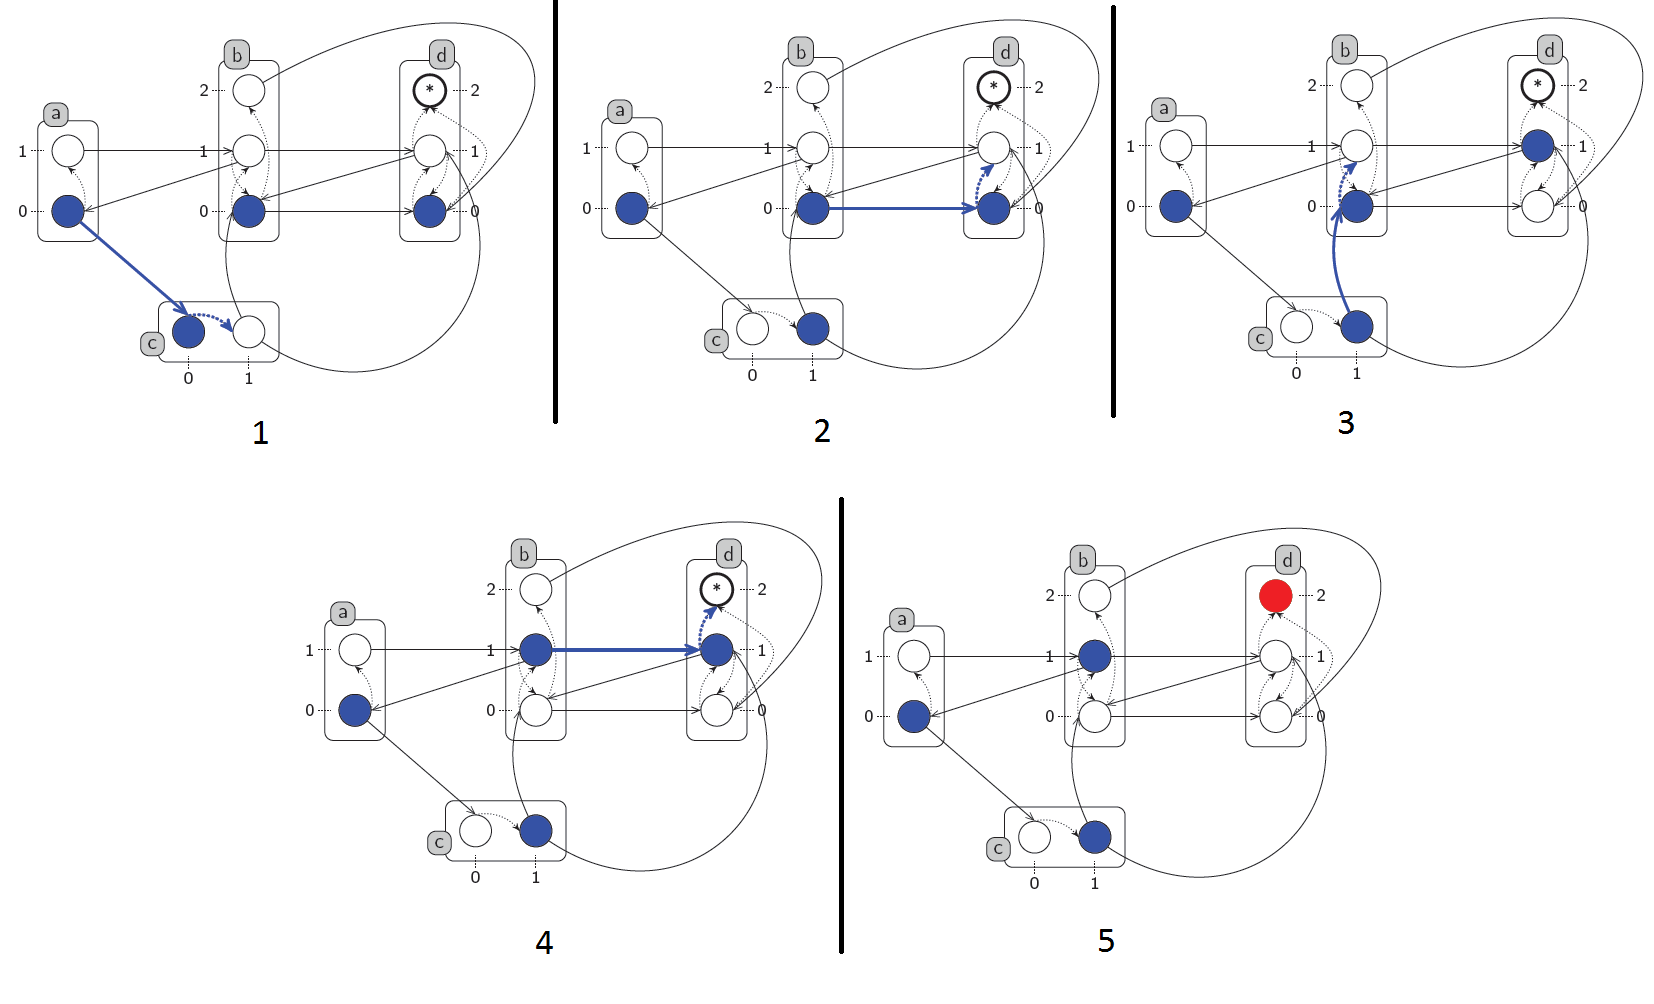
\includegraphics[width=0.95\textwidth]
    {./images/evolution.png}
    \caption{Exemple d'évolution du réseau de la figure \ref{fig:atteingnabiliteExp} vers le processus objectif $d_2$ aprés 4 changements. La successions des actions à partir de l'état initial $<a_0, b_0, c_0, d_0>$ est: $\PHfrappe{a_0}{c_0}{c_1}$:: $\PHfrappe{b_0}{d_0}{d_1}$:: $\PHfrappe{c_1}{b_0}{b_1}$ :: $\PHfrappe{b_1}{d_1}{d_2}$. Ainsi l'état final $<a_0, b_1, c_1, d_2>$ vérifie l'activation de $d_2$}
    \label{evolution}
\end{figure}